% !TeX root = ../main.tex
\chapter{Unidad 9: Factores que afectan la propagación del sonido}

\section*{Objetivo pedagógico}
\noindent\textbf{Objetivo.} Comprender cómo la distancia, la direccionalidad de la fuente, las condiciones atmosféricas y las interacciones con superficies alteran la propagación del sonido, y aplicar estos conocimientos al diseño de espacios clínicos (como cabinas audiométricas) y al control de ruido ambiental en fonoaudiología. Se incluyen ejemplos clínicos, actividades prácticas, recursos multimedia y ejercicios de autoevaluación.

\noindent\textbf{Pregunta inicial.} ¿Por qué un sonido se escucha más débil a mayor distancia? ¿Cómo afecta el viento o una pared al sonido en una cabina audiométrica? ¡Esta unidad te ayudará a entender cómo viaja el sonido!

\section{Distancia a la fuente}

\subsection{Ley del cuadrado inverso}
En un campo libre (sin reflexiones), el nivel de presión sonora (SPL) disminuye 6 dB cada vez que se duplica la distancia desde la fuente:
\[
L_{p2} = L_{p1} - 20 \log_{10}\left(\frac{d_2}{d_1}\right).
\]
Esto se debe a que la energía se distribuye en una esfera más grande, como ondas en un estanque.

\begin{quote}
    \textbf{Ejemplo clínico.} En una audiometría de campo libre, un tono de 90 dBSPL a 0.5 m se reduce a 78 dBSPL a 1 m, lo que afecta la calibración del audiómetro según la distancia al paciente.
\end{quote}

\begin{figure}[h]
    \centering
    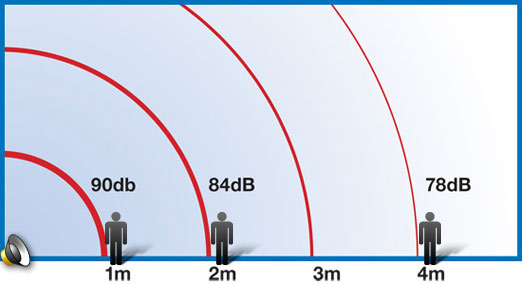
\includegraphics[width=0.9\textwidth]{figures/cuadrado_inverso.png}
    \caption{Representación de la ley del cuadrado inverso.}
    \label{fig:cuadrado-inverso}
\end{figure}


\section{Direccionalidad y factor \texorpdfstring{$Q$}{Q}}

\subsection{Definición}
El factor de directividad ($Q$) mide cómo una fuente concentra el sonido en una dirección:
\[
L_p = L_0 + 10 \log_{10} Q - 20 \log_{10}\left(\frac{d}{d_0}\right).
\]
Un $Q$ alto (como en una bocina) enfoca el sonido, aumentando el SPL en la dirección principal.

\begin{table}[h]
    \centering
    \begin{tabular}{|l|c|}
        \hline
        \textbf{Fuente} & \textbf{$Q$ aproximado} \\
        \hline
        Omnidireccional & 1 \\
        Hemiesférica (sobre suelo) & 2 \\
        Bocina direccional & 10–16 \\
        Line-array (banda media) & 30+ \\
        \hline
    \end{tabular}
    \caption{Valores típicos de directividad.}
\end{table}

\begin{quote}
    \textbf{Ejemplo clínico.} En una cabina audiométrica, se usan parlantes omnidireccionales ($Q=1$) para garantizar un campo sonoro uniforme, evitando variaciones por la posición del paciente.
\end{quote}

\begin{figure}[h]
    \centering
    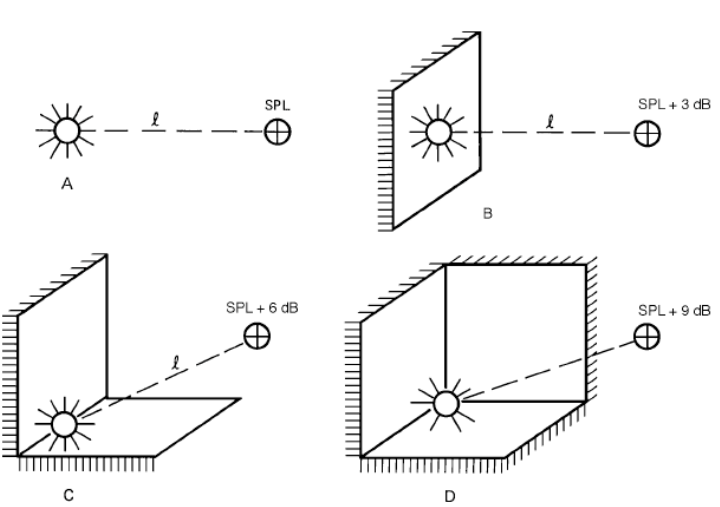
\includegraphics[width=0.9\textwidth]{figures/directividad.png}
    \caption{Diagrama de directividad de una fuente y cómo esta afecta a la propagación de la onda para $Q=1$, $Q=2$, $Q=3$ y $Q=4$}
    \label{directividad}
\end{figure}


\section{Condiciones atmosféricas}

\subsection{Temperatura}
La velocidad del sonido en el aire aumenta con la temperatura:
\[
c = 331 + 0.6T \, (\text{m/s}, \, T \text{ en °C}).
\]
Por ejemplo, a 30°C, $c \approx 349$ m/s. Los gradientes térmicos (como una inversión nocturna) curvan las ondas sonoras, aumentando el alcance al refractarlas hacia el suelo.

\begin{quote}
    \textbf{Ejemplo clínico.} En una evaluación de ruido ambiental cerca de una clínica, una inversión térmica nocturna puede hacer que el ruido de tráfico sea más audible, afectando las mediciones audiométricas.
\end{quote}

\subsection{Viento}
El viento modifica la velocidad efectiva del sonido:
\[
c' = c + u \cos \theta,
\]
donde $u$ es la velocidad del viento y $\theta$ el ángulo respecto al receptor. A favor del viento, el SPL aumenta; en contra, se reduce.

\subsection{Presión/altitud}
A mayor altitud, la menor densidad del aire reduce ligeramente el SPL (~1 dB por 1000 m).

\begin{quote}
    \textbf{Ejemplo clínico.} En una audiometría realizada a 2000 m de altitud, los niveles de salida de los auriculares pueden ser 2 dB más bajos, afectando la calibración del equipo y los resultados de la prueba.
\end{quote}

\section{Interacción con superficies}

\subsection{Reflexión y absorción}
Las superficies reflejan o absorben el sonido según su \textbf{coeficiente de absorción} ($\alpha$, de 0 a 1). La reverberación ($RT_{60}$, tiempo para que el sonido decaiga 60 dB) depende de la fórmula de Sabine:
\[
RT_{60} = \frac{0.161 V}{A}, \quad A = \sum (\alpha_i S_i),
\]
donde $V$ es el volumen del recinto y $A$ la absorción total.

\begin{quote}
    \textbf{Ejemplo clínico.} En una cabina audiométrica, se usan materiales absorbentes ($\alpha \approx 0.9$) para minimizar la reverberación, asegurando un campo libre.
\end{quote}

\subsection{Refracción}
El cambio de velocidad del sonido entre medios (por ejemplo, aire a vidrio) desvía las ondas, afectando el aislamiento en ventanas dobles.

\subsection{Difracción}
Las ondas rodean obstáculos si su tamaño es mucho menor que la longitud de onda ($\lambda$). Las frecuencias bajas (largas $\lambda$) difractan más, mientras que las altas quedan en sombra.

\begin{quote}
    \textbf{Ejemplo clínico.} En una clínica, una pared delgada no bloquea los graves (125 Hz, $\lambda \approx 2.7$ m), pero sí los agudos (4 kHz, $\lambda \approx 0.09$ m), afectando el aislamiento.
\end{quote}

\begin{figure}[h]
    \centering
    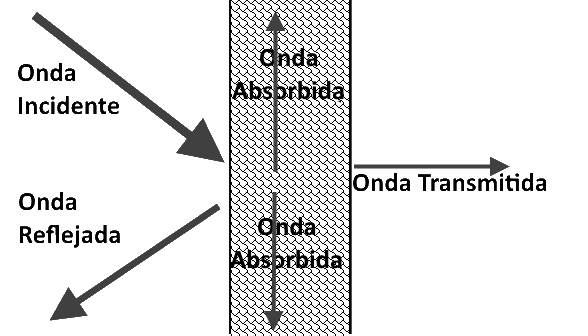
\includegraphics[width=0.9\textwidth]{figures/reflexion_absorcion.png}
    \caption{Fenómeno de reflexión y absorción de una onda sonora sobre una superficie.}
    \label{reflexion_absorcion}
\end{figure}

\section{Aislamiento e insonorización}
\begin{description}
    \item[\textbf{Aislamiento:}] Reduce la transmisión de sonido entre recintos, según la \textbf{ley de masas}:
    \[
    R \, (\text{dB}) = 20 \log_{10} (m f) - 47,
    \]
    donde $m$ es la masa superficial (kg/m²) y $f$ la frecuencia (Hz).
    \item[\textbf{Insonorización:}] Combina aislamiento y absorción para minimizar el ruido residual.
\end{description}

\begin{quote}
    \textbf{Ejemplo clínico.} Una cabina audiométrica requiere un aislamiento $>$70 dB a 1 kHz y un ruido residual $<$30 dBA para pruebas precisas.
\end{quote}

\section{Ejemplos prácticos}
\begin{enumerate}
    \item \textbf{SPL a distancia.} Un altavoz con $Q=4$ produce 90 dB a 2 m. A 8 m:
    \[
    L_p = 90 + 10 \log_{10} 4 - 20 \log_{10} \left(\frac{8}{2}\right) \approx 90 + 6 - 12 = 84 \, \text{dB}.
    \]
    \item \textbf{Velocidad y longitud de onda.} A 0°C, $c = 331$ m/s; a 30°C, $c = 349$ m/s. Para 500 Hz:
    \[
    \lambda_0 = \frac{331}{500} \approx 0.66 \, \text{m}, \quad \lambda_{30} = \frac{349}{500} \approx 0.70 \, \text{m}.
    \]
    \item \textbf{Altura de barrera.} Para atenuar 10 dB a 1 kHz ($\lambda \approx 0.34$ m), la barrera debe bloquear la línea de vista a 6 m. Usando la fórmula de difracción, altura mínima $\approx$1.5 m.
\end{enumerate}

\section{Ejercicios de autoevaluación}
\begin{enumerate}
    \item Explica por qué los sonidos graves (125 Hz) atraviesan paredes más fácilmente que los agudos (4 kHz).
    \item Describe cómo una inversión térmica nocturna aumenta el ruido de una fábrica en una clínica cercana.
    \item Calcula $RT_{60}$ para un aula de $8 \times 6 \times 3$ m ($V = 144$ m³) con $\bar{\alpha} = 0.25$. (\emph{Solución:} $RT_{60} \approx 0.72$ s.)
    \item Usa Decibel X para medir el ruido en una sala. Si supera 35 dBA, sugiere materiales absorbentes para reducir la reverberación.
\end{enumerate}

\section{Recursos recomendados}
\begin{itemize}
    \item Video: \href{https://www.youtube.com/watch?v=d8bODvda0NE&ab_channel=RyanHarne}{``Engineering Acoustics: 15. Outdoor Sound Propagation''}.
    \item App: Decibel X (gratis). Mide niveles de ruido.
    \item App: Tone Generator (gratis). Genera tonos para probar propagación.
    \item Libro: M. Raichel, \emph{Science and Applications of Acoustics}, capítulo 6.
    \item Norma: ISO 1996-2 (Medición de ruido ambiental).
\end{itemize}

\section*{Glosario}
\begin{description}
    \item[\textbf{$RT_{60}$:}] Tiempo para que el sonido decaiga 60 dB.
    \item[\textbf{$Q$:}] Factor de directividad, mide el enfoque del sonido.
    \item[\textbf{Sabine:}] Unidad de absorción (1 m² con $\alpha = 1$).
    \item[\textbf{Inversión térmica:}] Capa de aire caliente que refracta el sonido hacia el suelo.
\end{description}

\section*{Resumen}
\begin{itemize}
    \item \textbf{Distancia:} La ley del cuadrado inverso reduce el SPL 6 dB al duplicar la distancia.
    \item \textbf{Direccionalidad:} El factor $Q$ determina el enfoque del sonido.
    \item \textbf{Condiciones atmosféricas:} Temperatura, viento y altitud afectan la velocidad y el SPL.
    \item \textbf{Superficies:} Reflexión, absorción y difracción modifican el sonido.
    \item \textbf{Aislamiento:} La ley de masas y la insonorización son clave en cabinas audiométricas.
\end{itemize}


\bigskip
\noindent\emph{Conclusión.} Comprender cómo la distancia, la direccionalidad, las condiciones ambientales y las superficies afectan el sonido es esencial para diseñar cabinas audiométricas, optimizar la inteligibilidad del habla y controlar el ruido en entornos clínicos.



%%%%%%%%%%%%%%%%%%%%%%%%%%%%%%%%%%%%%%%%%%%%%%%%%%%%%%%%%%%%%%%%%%%%%%%%%%%%%%%%%%%%%%%%%%%%%%%%%%
